% Gemini theme
% https://github.com/anishathalye/gemini

\documentclass[final]{beamer}

\usepackage[T1]{fontenc}
\usepackage{lmodern}

\usepackage[size=custom,width=101.6,height=81.28,scale=1.0]{beamerposter}
\usetheme{gemini}
\usecolortheme{cwru}

\usepackage[numbers, sort&compress]{natbib}

\usepackage{amsmath, amssymb}

\expandafter\def\expandafter\normalsize\expandafter{%
    \normalsize%
    \setlength\abovedisplayskip{10pt}%
    \setlength\belowdisplayskip{10pt}%
    \setlength\abovedisplayshortskip{10pt}%
    \setlength\belowdisplayshortskip{10pt}%
}

\usepackage{graphicx}
\usepackage[caption=false]{subfig}
\usepackage{capt-of}

\usepackage{booktabs}

\usepackage{tikz}
\usetikzlibrary{bayesnet, plotmarks, matrix}

\usepackage{pgfplotstable}
\usepackage{pgfplots}
\usepgfplotslibrary{groupplots, statistics}
\pgfplotsset{compat=1.15}
% Box plots
\pgfplotsset{
	only if/.style args={entry of #1 is #2}{
		/pgfplots/boxplot/data filter/.code={
			\edef\tempa{\thisrow{#1}}
			\edef\tempb{#2}
			\ifx\tempa\tempb
			\else
			\def\pgfmathresult{}
			\fi
		}
	}
}

% If you have N columns, choose \sepwidth and \colwidth such that
% (N+1)*\sepwidth + N*\colwidth = \paperwidth
\newlength{\sepwidth}
\newlength{\colwidth}
\setlength{\sepwidth}{0.025\paperwidth}
\setlength{\colwidth}{0.3\paperwidth}

\newcommand{\separatorcolumn}{\begin{column}{\sepwidth}\end{column}}

\newcommand{\vTransmissionRate}{\alpha}
\newcommand{\vSendCoefficient}{\gamma}
\newcommand{\vTimeBuffer}{\beta}
\newcommand{\vScore}{s}

\newcommand{\vVariable}[1]{v_{#1}}
\newcommand{\vFactor}[2]{f_{#1#2}}
\newcommand{\vVariables}{V}
\newcommand{\vPath}{P}

\newcommand{\vReachability}{m}
\newcommand{\vEstimatedReachability}{\hat{\vReachability}}

\newcommand{\twodots}{\mathinner {\ldotp \ldotp}}

\title{ShareTrace: Contact Tracing with the Actor Model}

\author{Ryan Tatton \and Erman Ayday \and Youngjin Yoo \and Anisa Halimi}

\institute[shortinst]{Case Western Restern Reserve University}

\footercontent{
  \href{https://github.com/share-trace}{https://github.com/cwru-xlab} \hfill
  Pandemic Preparedness Workshop 2023 \hfill
  \href{mailto:ryan.tatton.edu}{ryan.tatton@case.edu}}

\begin{document}
\begin{frame}[t]
\begin{columns}[t]
\separatorcolumn
\begin{column}{\colwidth}
	\begin{block}{1. Motivation}
		\begin{itemize}
			\item Proximity-based contact tracing relies on mobile-device interaction to estimate infection spread.
			\item ShareTrace is a privacy-preserving, proximity-based contact-tracing solution that estimates a user's infection risk (\emph{exposure score}) via message passing on a factor graph based on their prior probability of infection (\emph{symptom score}) and (in)direct contact with others.
			\item The scalability and efficiency of the original, synchronous ShareTrace algorithm (\emph{risk propagation}) \cite{Ayday2021} can be improved with asynchronous message passing on a temporal contact network.
		\end{itemize}
	\end{block}
	\begin{block}{2. Proposed Scheme}
		\begin{itemize}
			\item Reformulate the factor graph as a contact network (Figure \ref{fig:contact-network}) and partition the network into subnetwork \emph{actors} \cite{Agha1986} that pass messages (i.e., risk scores) asynchronously until convergence.
			\item Only propagate risk scores if they are likely to affect other users' exposure scores in the network.
			\item The \emph{send coefficient} $\vSendCoefficient$ parametrizes the accuracy-efficiency trade-off of asynchronous message passing: an actor only propagates a risk score if it is sufficiently high (by a factor of $\vSendCoefficient$) and sufficiently old (relative to its initial message).
			\item Guaranteed convergence for $\vTransmissionRate < 1$ and $\vSendCoefficient > 0$.
		\end{itemize}
		\begin{figure}
			\centering
			\resizebox{0.75\columnwidth}{!}{%
				\begin{tikzpicture}[baseline={(0,0)}, ampersand replacement=\&]
					\matrix[row sep=1em] at  (-4, 0)
					{%
						\& \factor[minimum size=0.5em] {f12} {above:$\vFactor{1}{2}$} {} {}; \&\&
						\factor[minimum size=0.5em] {f23} {above:$\vFactor{2}{3}$} {} {}; \& \\
						\node[latent, label=below:$\vVariable{1}$, minimum size=1em] (v1) {}; \&\&
						\node[latent, label=below:$\vVariable{2}$, minimum size=1em] (v2) {}; \&\&
						\node[latent, label=below:$\vVariable{3}$, minimum size=1em] (v3) {}; \\
					};
					\edge[-] {v1} {f12};
					\edge[-] {v2} {f12};
					\edge[-] {v2} {f23};
					\edge[-] {v3} {f23};
					$\implies$
					\matrix[row sep=3em, column sep=2em] at (6, 0)
					{%
						\node[latent, label=below:$\vVariable{1}$, minimum size=1em] (v1) {}; \&
						\& \node[latent, label=below:$\vVariable{3}$, minimum size=1em] (v3) {}; \\
						\& \node[latent, label=below:$\vVariable{2}$, minimum size=1em] (v2) {}; \& \\
					};
					\factor[minimum size=0.5em, above= of v1] {f121} {above:$\vFactor{1}{2}$} {} {};
					\factor[minimum size=0.5em, above= of v2, xshift=-1.5em] {f122} {above:$\vFactor{1}{2}$} {} {};
					\factor[minimum size=0.5em, above= of v2, xshift=1.5em] {f232} {above:$\vFactor{2}{3}$} {} {};
					\factor[minimum size=0.5em, above= of v3] {f233} {above:$\vFactor{2}{3}$} {} {};

					\plate[inner sep=0.3em, yshift=-0.4em] {p1} {(v1)(f121)(f121-caption)} {};
					\plate[inner sep=0.3em, yshift=-0.4em] {p2} {(v2)(f122)(f232)(f122-caption)(f232-caption)} {};
					\plate[inner sep=0.3em, yshift=-0.4em] {p3} {(v3)(f233)(f233-caption)} {};

					\edge[-] {v1} {f121};
					\edge[-] {v2} {f122};
					\edge[-] {v2} {f232};
					\edge[-] {v3} {f233};
					\edge[-] {p1} {p2};
					\edge[-] {p2} {p3};
				\end{tikzpicture}
			}%
			\caption{A factor graph of 3 variables and 2 factors (left) as a contact network of 3 users (right).}
			\label{fig:contact-network}
		\end{figure}
	\end{block}
    \begin{block}{3. Message Reachability (MR)}
        \begin{itemize}
            \item A \emph{time-respecting path} is a sequence of nondecreasing contacts in a contact network; vertex $v$ is \emph{temporally reachable} from vertex $u$ if a path from $u$ to $v$ exists.
            \item Generalize temporal reachability to account for message-passing semantics: \emph{MR from vertex $u$ to vertex $v$} along the shortest path $\vPath$ where $f(u, i, j, v) = 1$ if all constraints are satisfied and $f(u, i, j, v) = 0$ otherwise:
                \begin{equation*}
                    \vReachability(u, v) = \sum_{(i, j) \in \vPath} f(u, i, j, v) \qquad \vReachability(u) = \max \{\vReachability(u, v) \mid v \in \vVariables \}
                \end{equation*}
            \item Let $H(x)$ be the \emph{Heaviside function} and enumerate the path vertices $[0 \twodots |\vPath| - 1]$.
                \begin{equation*}
                    \vReachability(u) = \underset{\vPath}{\max} \left\{\sum_{(i, j) \in \vPath} H(t_{ij} + \vTimeBuffer - t_u) \cdot H(\vTransmissionRate^i \cdot \vScore_u - \vSendCoefficient \cdot \vScore_i) \cdot H(t_i - t_u) \right\}
                \end{equation*}
                where $\vScore_i$ ($t_i$) is the initial risk score (time) of user $i$, $t_{ij}$ is the latest contact time between users $i$ and $j$; and $\vTimeBuffer$ is a time buffer to account for reporting delay.
            \item \emph{Estimated MR of vertex $u$ to vertex $v$} relaxes the temporality constraints:
            	\begin{equation} \label{eq:msg-reach}
                    \vEstimatedReachability(u, v) &= \log_{\vTransmissionRate} \left\{\vSendCoefficient \cdot \frac{\vScore_v}{\vScore_u} \right\} \qquad
                    \vEstimatedReachability(u) &= \max \{\vEstimatedReachability(u, v) \mid v \in \vVariables \}
            	\end{equation}
            \item MR quantifies communication complexity, individual risk, and population risk.
		\end{itemize}
	\end{block}
\end{column}
\separatorcolumn
\begin{column}{\colwidth}
	\begin{block}{4. Experimental Design}
		\begin{itemize}
			\item Synthetic networks included random geometric graphs (RGG) \cite{Dall2002}, benchmark graphs (LFRG) \cite{Lancichinetti2008}, and clustered scale-free graphs (CSFG) \cite{Holme2002}. Figure \ref{fig:sociopatterns} visualizes real-world networks.
			\item METIS was used to partition the networks with a load imbalance factor of 0.2, set to attempt contiguous partitions, and minimize inter-partition connectivity \cite{Karypis1998}.
			\item Users were assigned "high" risk (scores above 0.5) with probability 0.2.
			\item Default parameter values: transmission rate $\vTransmissionRate = 0.8$; send coefficient $\vSendCoefficient = 0.6$.
			\item 10 trials for each synthetic (real-world) network for MR (scalability) experiments.
		\end{itemize}
		\vspace{-1em}
	    \begin{figure}
	    	\centering
	    	\subfloat[High school: 180 / 2,220]
	    		{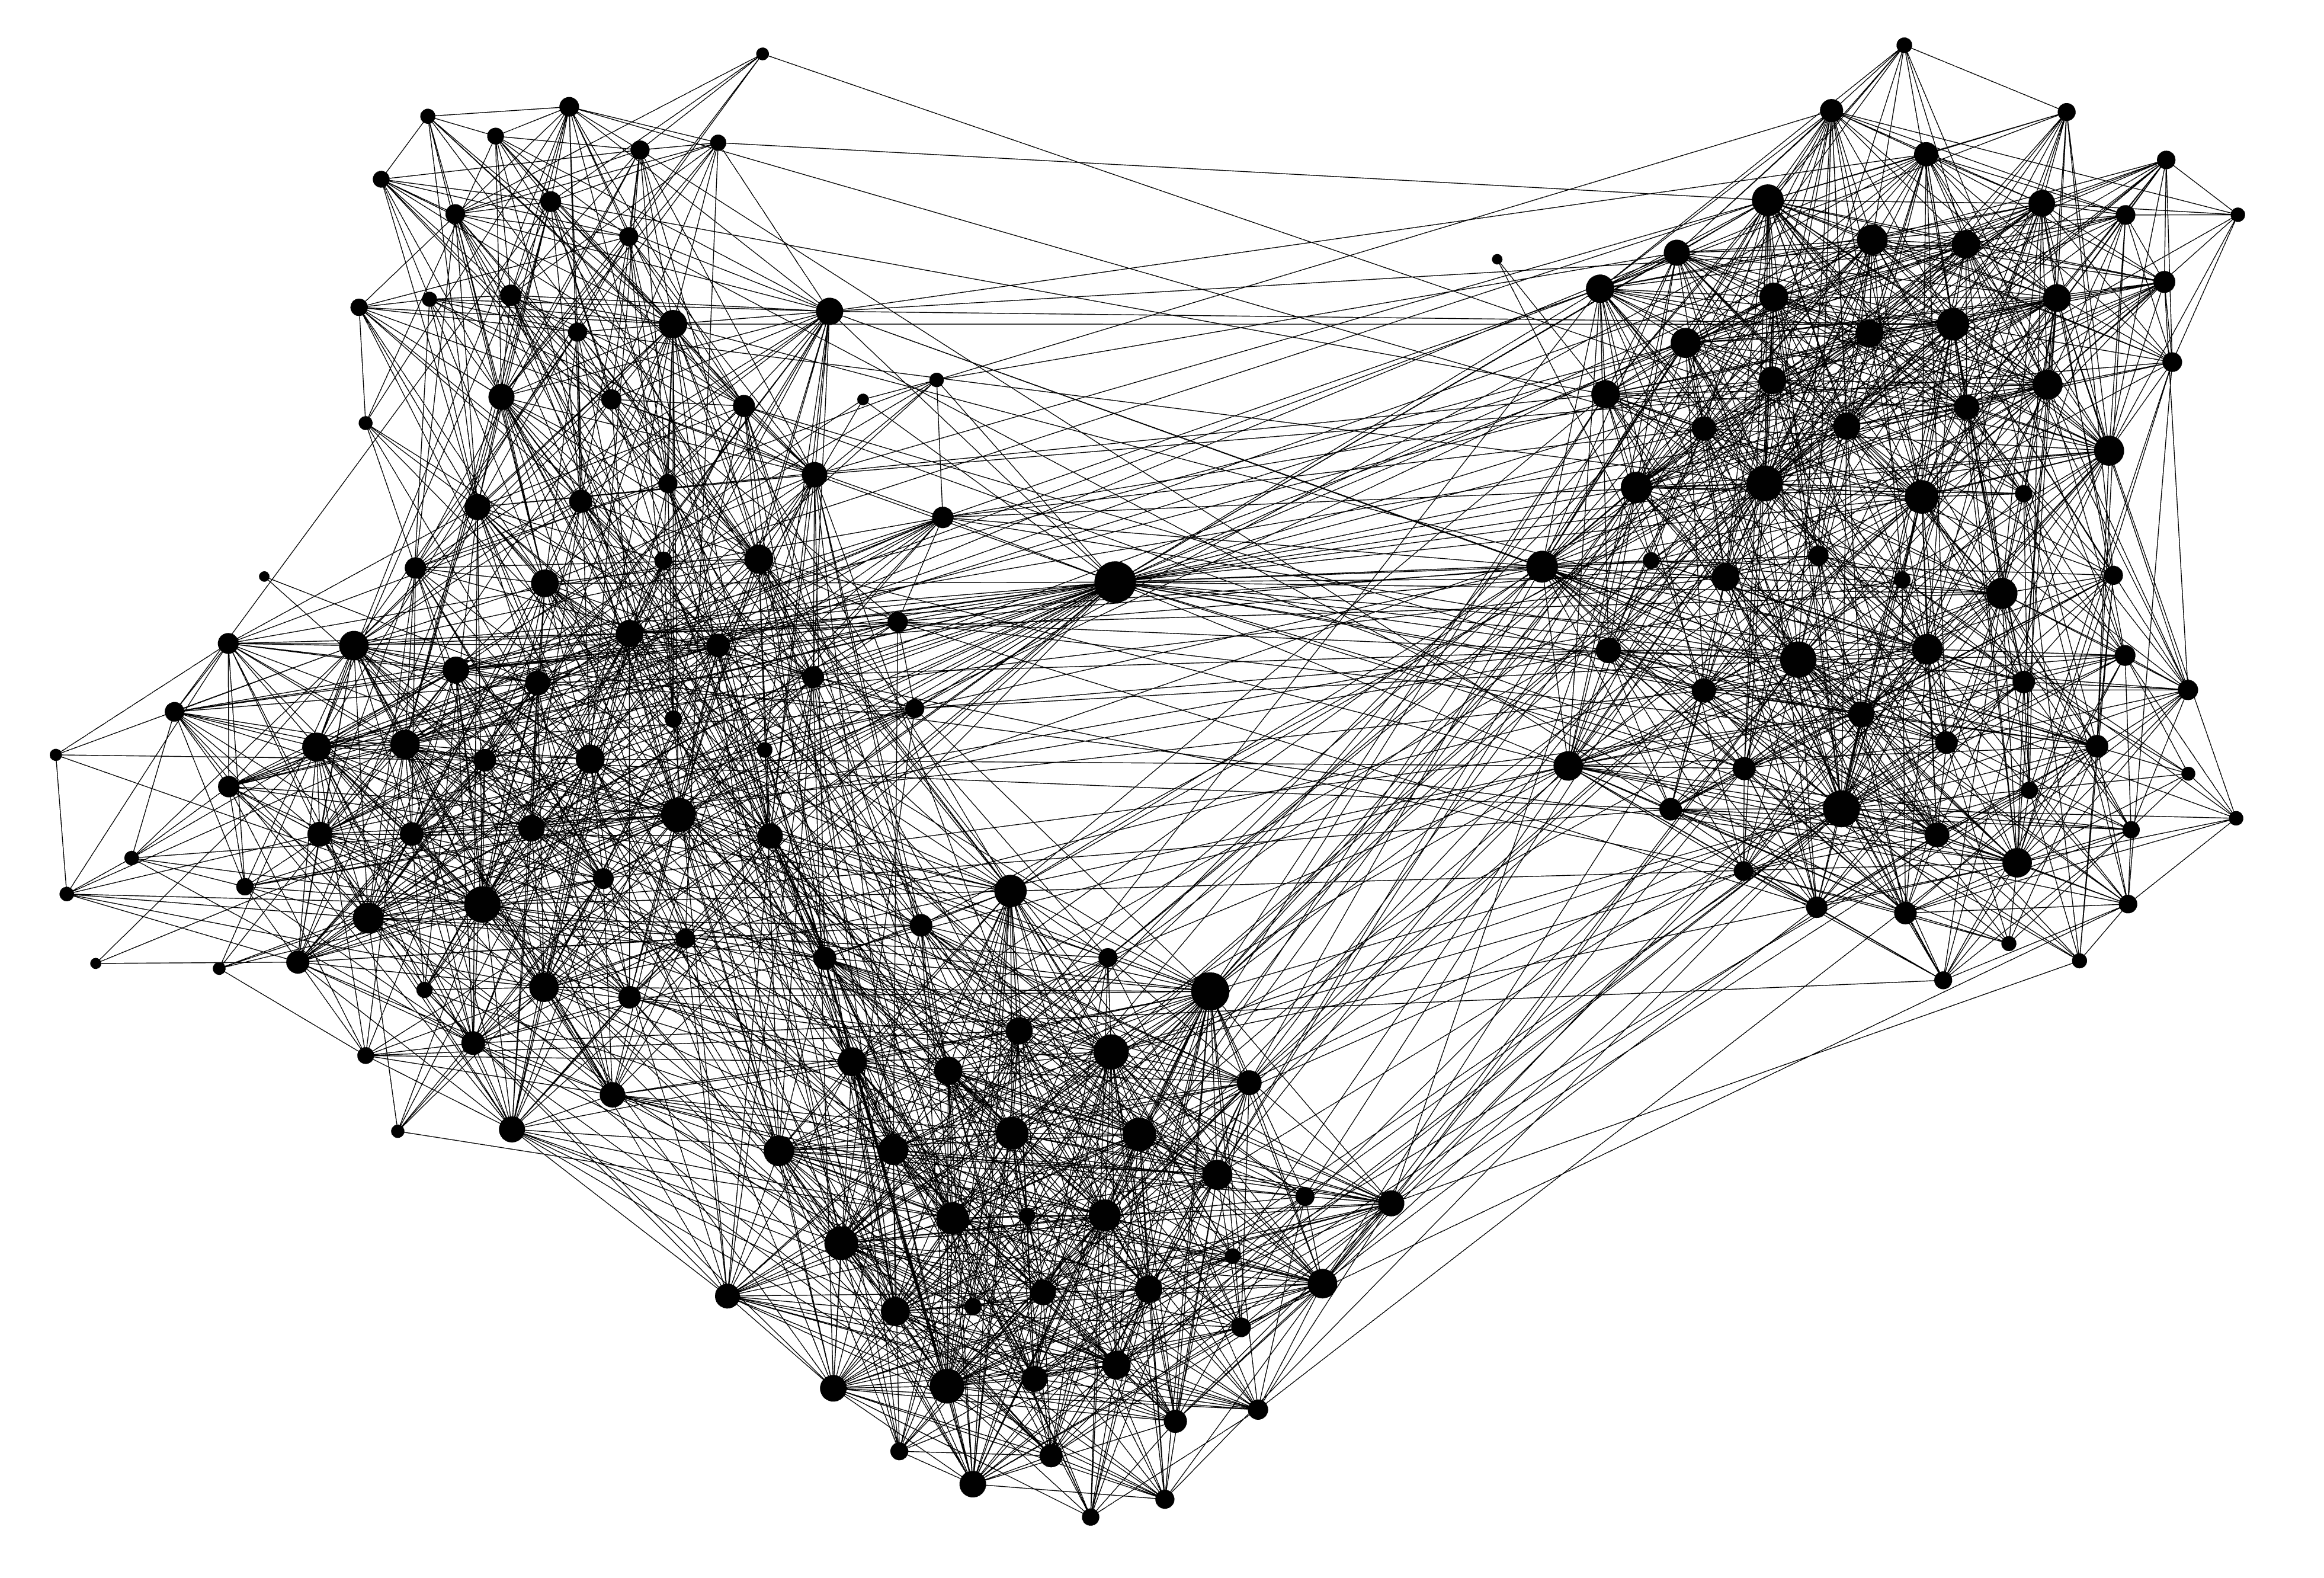
\includegraphics[width=0.35\columnwidth]{anc/highschool12}} \qquad
			\subfloat[Workplace: 217 / 4,274]
				{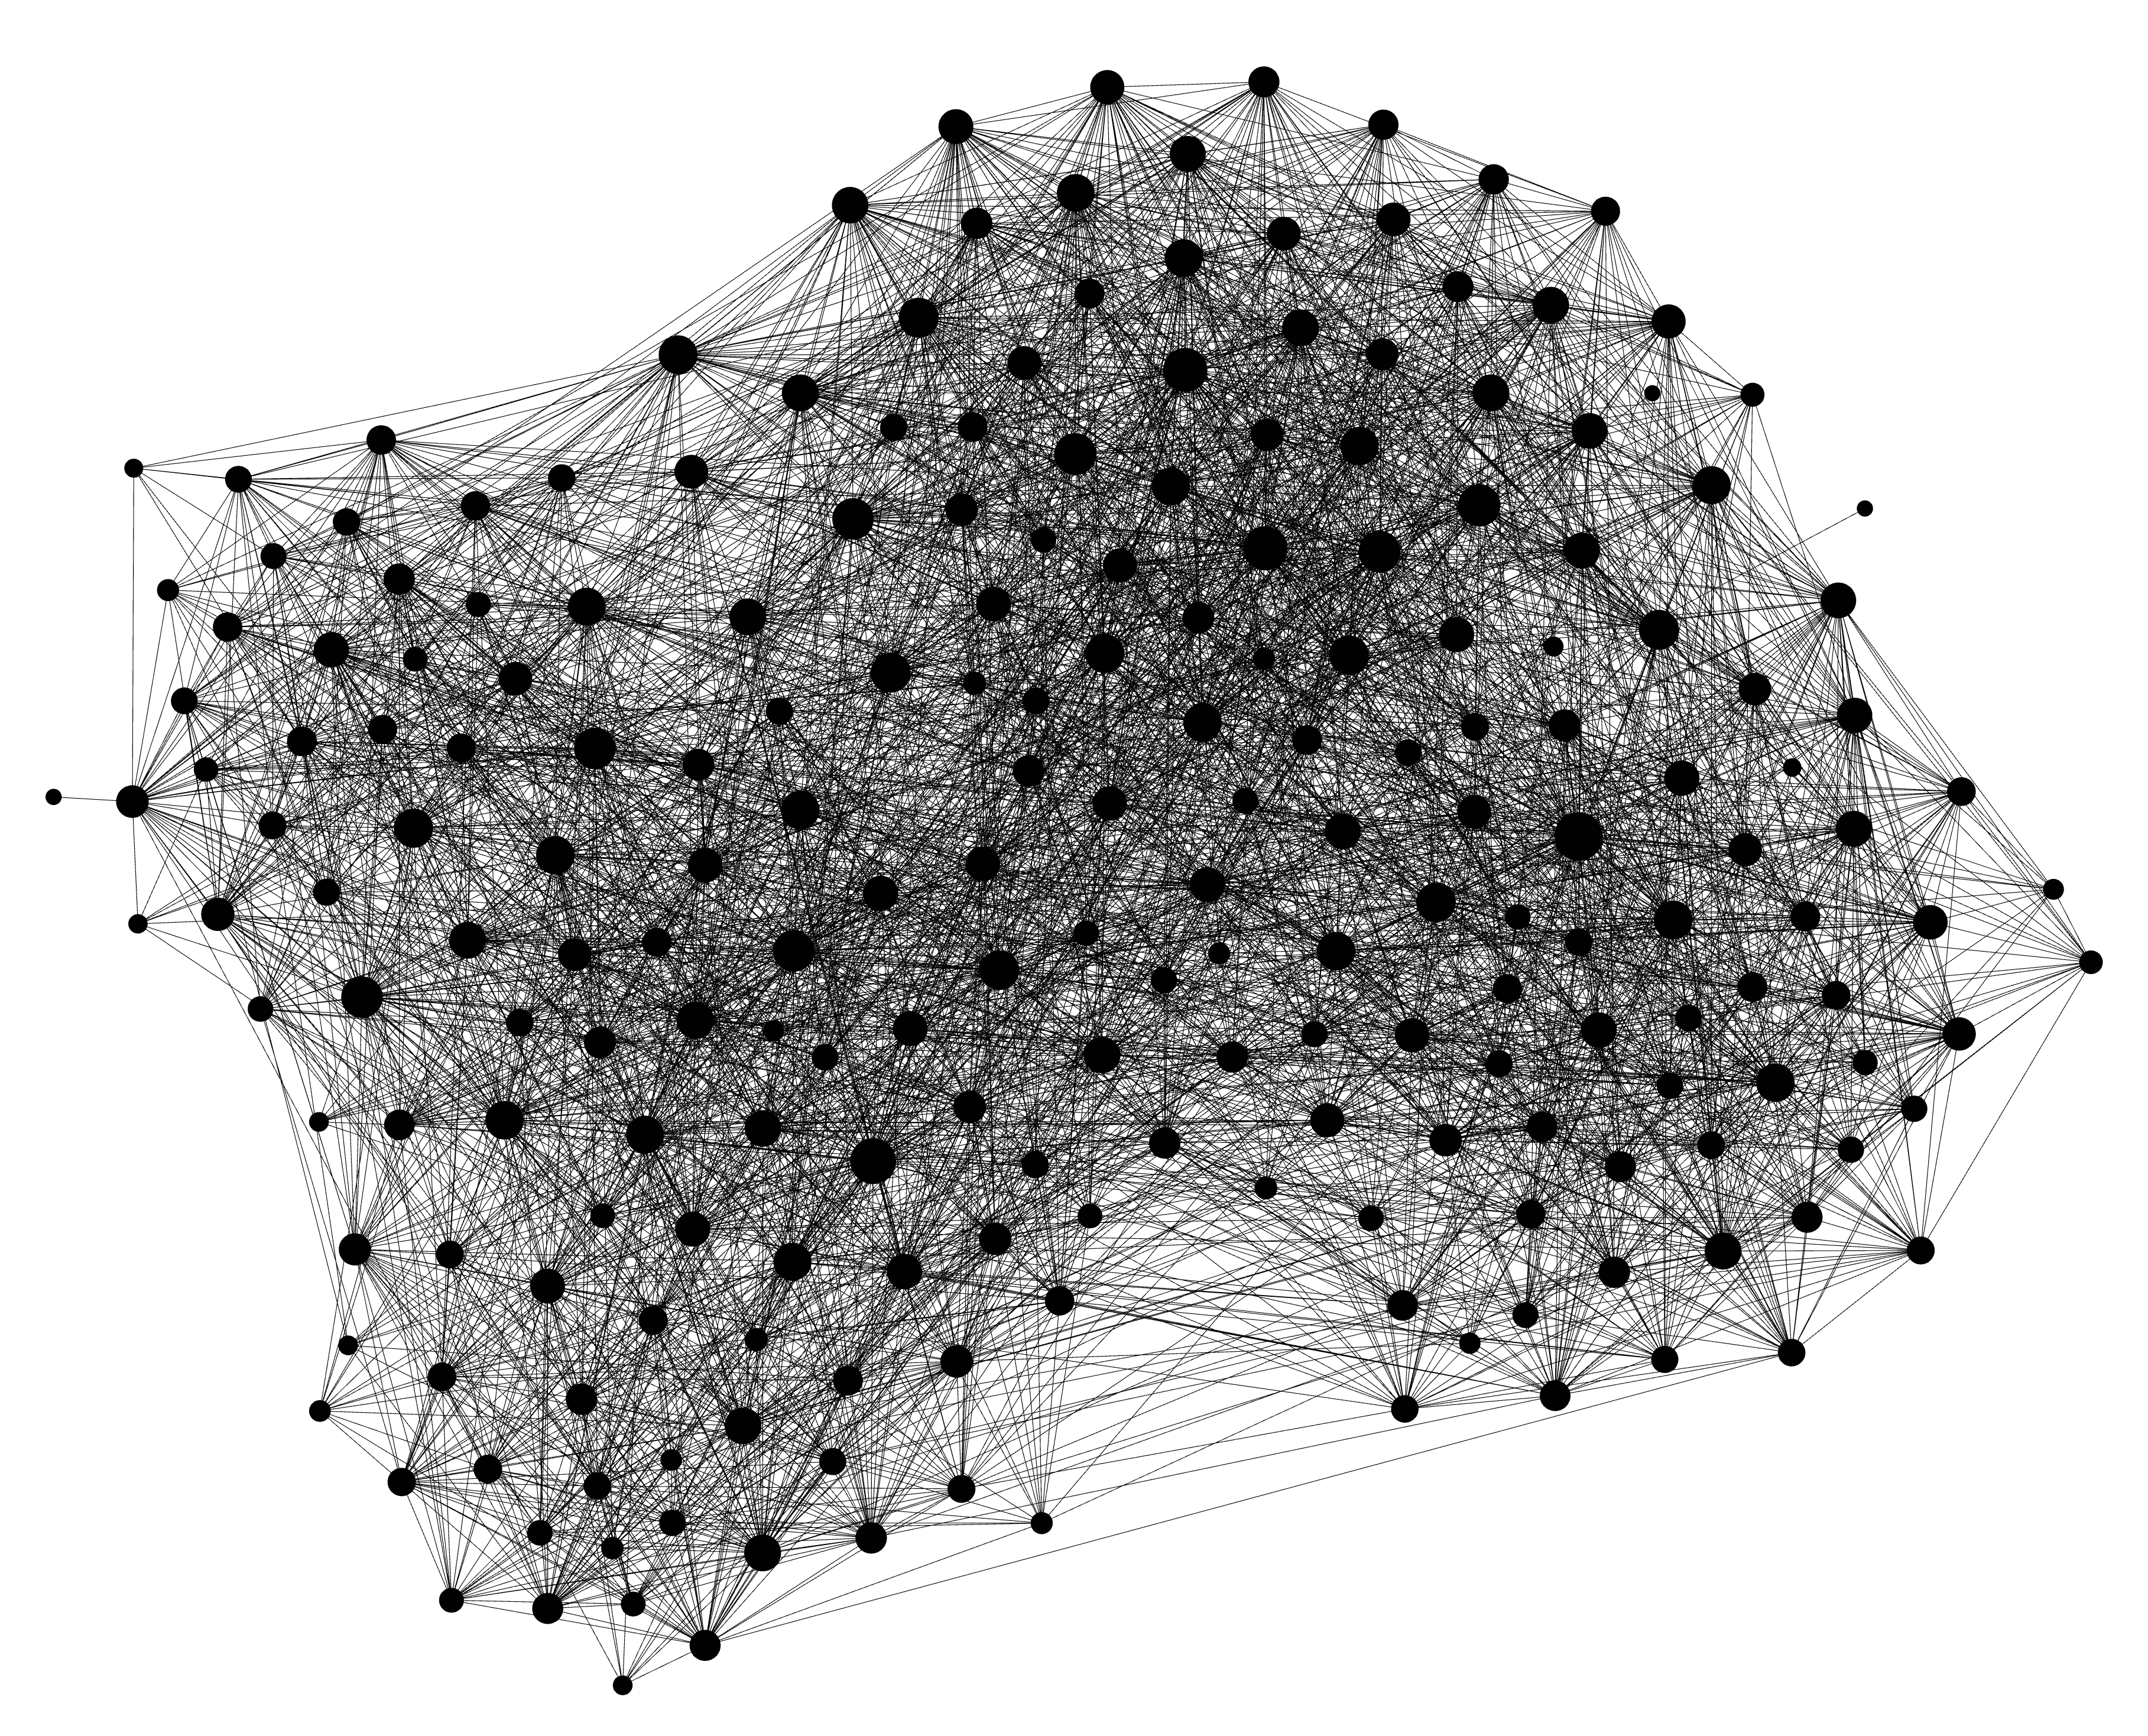
\includegraphics[width=0.35\columnwidth]{anc/workplace}} \qquad
			\subfloat[Scientific conference: 403 / 9,565]
				{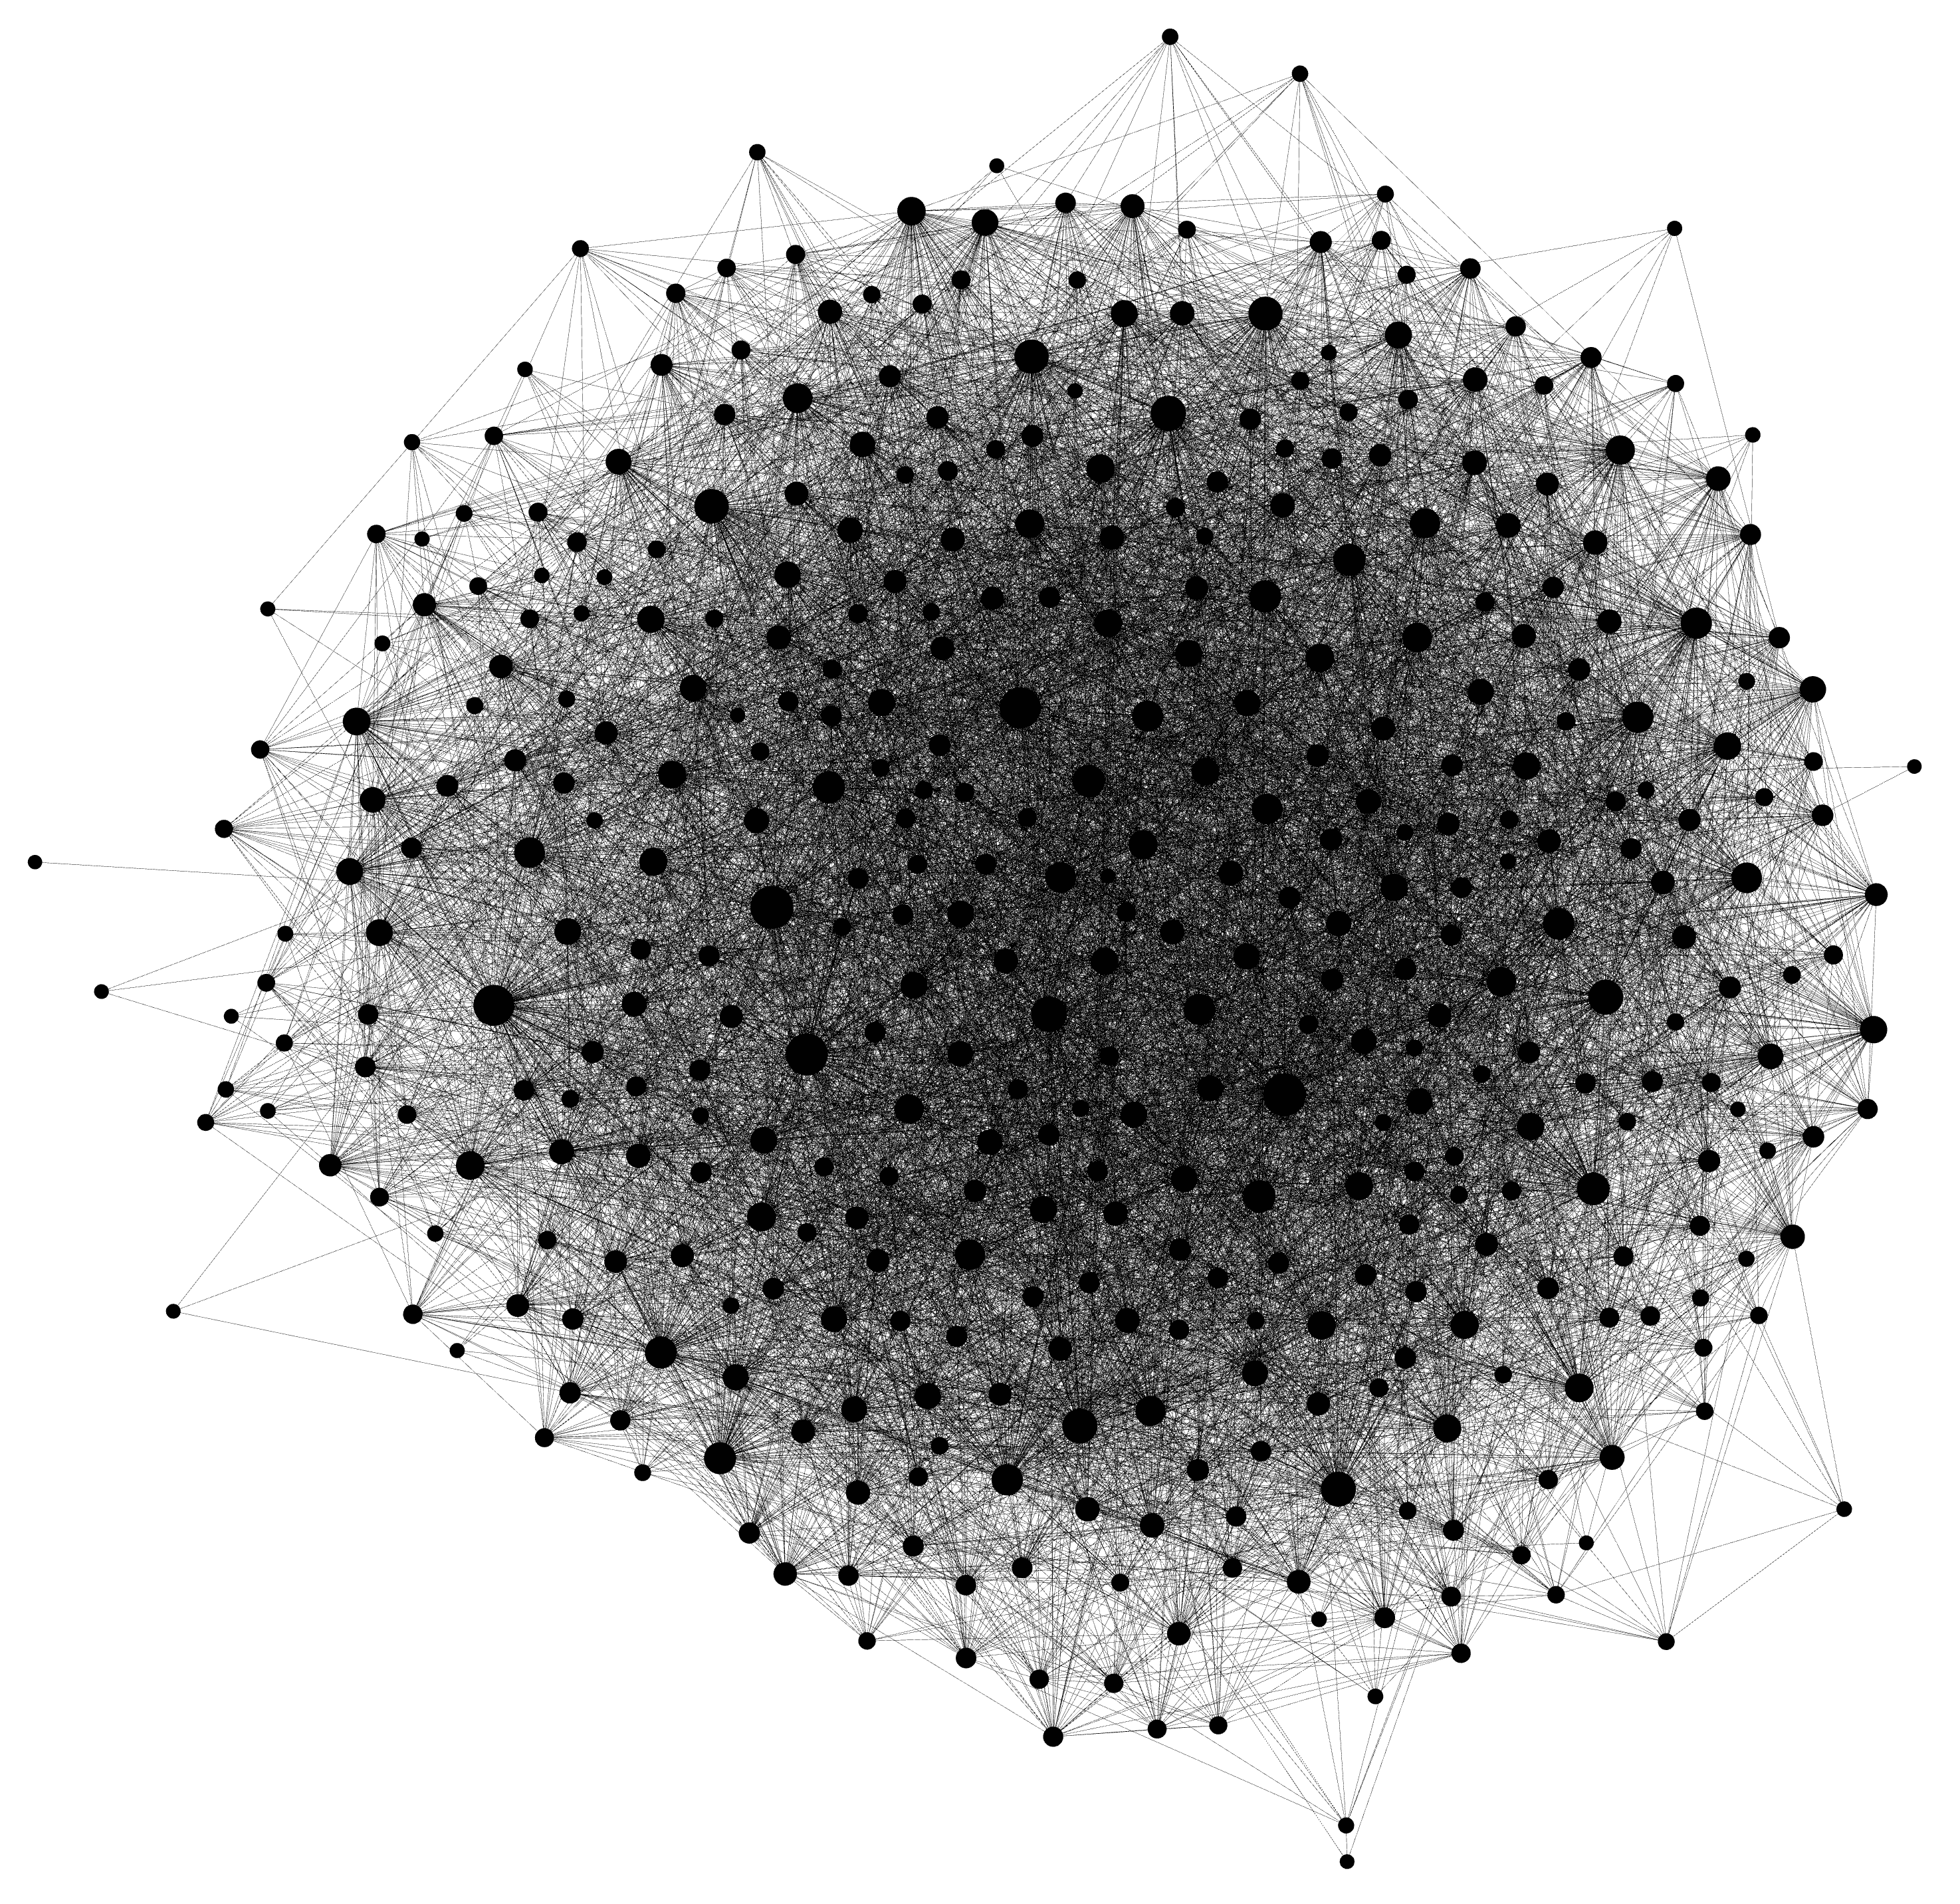
\includegraphics[width=0.35\columnwidth]{anc/conference}}
			\caption{SocioPatterns contact networks (number of users / number of contacts) \cite{Genois2018}. Each edge represents the most recent time of contact (duration of at least 20 seconds) between two users.}
			\label{fig:sociopatterns}
		\end{figure}
	\end{block}
	\begin{block}{5. Efficiency Results}
		\begin{itemize}
			\item Synthetic networks with 5,000 users and 2 actors were use to evaluate the effects of transmission rate and send coefficient on risk propagation efficiency.
			\item A send coefficient of $\vSendCoefficient = 0.6$ optimizes for accuracy and efficiency by permitting 99\% of the possible user updates, while resulting in faster runtimes, $(Q_1, Q_2, Q_3) = (0.13, 0.13, 0.46)$, and fewer messages, $(Q_1, Q_2, Q_3) = (0.13, 0.15, 0.44)$, for a transmission rate of $\vTransmissionRate = 0.8$.
		\end{itemize}
		\vspace{-1em}
		\begin{figure}
			\centering
			\resizebox{\columnwidth}{!}{%
				\begin{tikzpicture}
					\begin{groupplot}[
						group style={
						group size=3 by 1,
						xlabels at=edge bottom,
						y descriptions at=edge left
					},
					boxplot,
					table/col sep=comma,
					boxplot/draw direction=y,
					scaled x ticks={base 10:-1},
					width=0.3\columnwidth,
					height=0.35\columnwidth,
					ytick distance=0.2,
					xtick scale label code/.code={},
					xlabel={Send coefficient, $\vSendCoefficient$}
				]
					\nextgroupplot[table/y=NormalizedUpdates, title={Normalized updates}]
						\foreach \t in {1,...,10} {%
							\addplot[color=black] table[only if={entry of SendTolerance is \t}]
							{anc/tolerance-updates.csv};
						}%
					\nextgroupplot[table/y=NormalizedRuntimeInSeconds, title={Normalized runtime}]
						\foreach \t in {1,...,10} {%
							\addplot[color=black] table[only if={entry of SendTolerance is \t}]
							{anc/tolerance-runtime.csv};
						}%
						\nextgroupplot[table/y=NormalizedMessages, title={Normalized messages}]
						\foreach \t in {1,...,10} {%
							\addplot[color=black] table[only if={entry of SendTolerance is \t}]
							{anc/tolerance-messages.csv};
						}%
					\end{groupplot}
				\end{tikzpicture}
			}%
			\caption{Effects of send coefficient and transmission rate on efficiency. All dependent variables are normalized across networks and transmission rates. Efficiency on LFRGs were less sensitive to changes in transmission rate and send coefficient than RGGs and CSFGs, which is the cause for the large interquartile ranges.}
		\end{figure}
	\end{block}
\end{column}
\separatorcolumn
\begin{column}{\colwidth}
	\begin{block}{6. Message Reachability Results}
		\begin{itemize}
			\item Equation \eqref{eq:msg-reach} was a better estimator for synthetic networks than real-world networks (Table \ref{table:reach}).
			\item With lower (higher) send coefficients (transmission rates), \eqref{eq:msg-reach} suggests higher MR; however, a message is only passed under certain conditions, so \eqref{eq:msg-reach} tends to overestimate reachability.
		\end{itemize}
		\begin{table}
			\begin{minipage}[b]{0.66\columnwidth}
				\centering
					\begin{tikzpicture}
						\begin{groupplot}[
							group style={
								group size=2 by 1,
								xlabels at=edge bottom,
								y descriptions at=edge left
							},
							boxplot,
							title={A/E MRR, $\vReachability / \vEstimatedReachability$},
							table/col sep=comma,
							boxplot/draw direction=y,
							xtick distance=2,
							scaled x ticks={base 10:-1},
							xtick scale label code/.code={},
							ytick distance=0.5,
							width=0.5\columnwidth,
							height=0.65\columnwidth
							]
							\nextgroupplot[table/y=RatioValue, xlabel={Send coefficient, $\vSendCoefficient$}]
							\foreach \t in {1,...,10} {%
								\addplot[color=black] table[only if={entry of SendTolerance is \t}]
								{anc/ratio-tolerance.csv};
							}%
							\nextgroupplot[table/y=RatioValue, xlabel={Transmission rate, $\vTransmissionRate$},]
							\foreach \t in {1,...,9} {%
								\addplot[color=black] table[only if={entry of Transmission is \t}]
								{anc/ratio-transmission.csv};
							}%
						\end{groupplot}
					\end{tikzpicture}
				\captionof{figure}{Effects of send coefficient and transmission rate on actual/estimated MR ratio (A/E MRR) on synthetic and real-world networks.}
				\label{fig:ratios}
			\end{minipage}
			\hfill
			\begin{minipage}[b]{0.3\columnwidth}
				\centering
				\begin{tabular}{@{}lc@{}}
					\toprule
					Network & $\vReachability / \vEstimatedReachability \pm 1.96 \cdot \mathrm{SE}$ \\
					\midrule
					\emph{Synthetic} & \\
					LFR & $0.88 \pm 0.14$\\
					RGG & $0.74 \pm 0.12$\\
					CSFG & $0.90 \pm 0.14$\\
					& $\boldsymbol{0.85 \pm 0.08}$ \\
					\midrule
					\emph{Real-world} & \\
					Thiers13 & $0.58 \pm 0.01$\\
					InVS15 & $0.63 \pm 0.01$\\
					SFHH & $0.60 \pm 0.01$\\
					& $\boldsymbol{0.60 \pm 0.01}$\\
					\bottomrule
				\end{tabular}
				\caption{A/E MRR for synthetic and real networks ($\vTransmissionRate = 0.8$, $\vSendCoefficient = 0.6$). Synthetic (real-world) ratios are averaged across parameter combinations (trials).}
				\label{table:reach}
			\end{minipage}
		\end{table}
	\end{block}
	\begin{block}{7. Scalability Results}
		\begin{figure}
			\centering
			\begin{tikzpicture}
				\begin{axis}[
					width=0.6\columnwidth,
					height=0.4\columnwidth,
					xlabel={Contacts},
					title={Runtime (minutes)},
					ytick distance = 60,
					xtick distance=5e3,
					scaled y ticks={real:60},
					ytick scale label code/.code={}
					]
					\addplot[
						scatter,
						only marks,
						scatter src=explicit symbolic,
						scatter/classes={
							1={mark=x,blue},
							2={mark=+,orange},
							3={mark=o,draw=green}% no comma
						},
						mark size=3pt
					]
					table [col sep=comma,x=Edges,y=RuntimeInSeconds,meta=Graph]
					{anc/scalability.csv};
					\legend{LFRG,CSFG,RGG}
				\end{axis}
			\end{tikzpicture}
			\caption{Runtimes of risk propagation on synthetic networks (100–10,000 users; $\sim$200–38,000 contacts). A linear regression fit explains ($R^2 = 0.52$) the runtime of LFRGs and RGGs with slope $m = (1.1 \pm 0.1) \cdot 10^{-3}$ seconds/contact and intercept $b = 4.3 \pm 1.6$ seconds ($\pm 1.96 \cdot \mathrm{SE}$). The runtime behavior of CSFGs requires further investigation.}
			\label{fig:scalability}
		\end{figure}
		\vspace{-1em}
	\end{block}
	\begin{block}{Acknowledgements}
		Research was partly supported by the Cisco Research University Funding grant number 2800379.
	\end{block}
	\begin{block}{References}
		\nocite{*}
		\scriptsize{\bibliographystyle{abbrvnat}\bibliography{poster}}
	\end{block}
\end{column}
\separatorcolumn
\end{columns}
\end{frame}
\end{document}
